\section{Research Questions}
\label{section-research-questions}

My hypothesis is that using mobile analytics can help improve both the work development teams do and the quality of the product they create. Here work includes the development, bug investigation, and testing of the software being created. For the quality of the product I'm focusing on a subset of qualities, which are technology-centric.

I picked the domain of mobile apps as they are ubiquitous, extremely popular, and have interesting and challenging contexts of use. And within the range of mobile apps I ended up focusing on Android apps for various reasons including: the analytics tools available, the relative glut of suitable apps available to me, my prior experience and expertise, and their market share.

The core question I aim to consider is: 
\emph{How can applying analytics improve software development and software testing?} Here I am assuming that analytics can help, as stated by Buse and Zimmermann ~(\citeyear{buse_analytics_2010}); and \emph{``with explicit and implicit feedback now available (almost) continuously, questions arise. How can practitioners use this information and integrate it into their development processes [to decide when to release updates]?"}~\citep{maalej2016_towards_data_driven_requirements_engineering}.

This leads to several related questions that underpin this main question \emph{i.e.}, I have grouped these in three categories: sources, value, and impact.

\akb{There are a lot of sub-questions below. You will need to focus on the ones you have data to evaluate, or have more abstract formulations that cover groups of sub-questions.}

\yijun{If possible, you may need to dig out a few MobileSoft research papers to give evidence that these research questions have not been addressed in literature, e.g., \emph{Future Trends in Software Engineering Research for Mobile Apps}~\citep{nagappan2016_future_trends_in_sw_eng_for_mobile_apps}, whether the future work of some paper suggests one does not know the sources, value, or impact of mobile analytics to assess and improve app quality? Is there nothing in the general SE literature studying the "analytics" to "general software quality" problem? If there are such general work, how does "mobile analytics" and "app quality" differentiate the RQs to existing ones...}

\begin{mdframed}[style=MyFrame]
\emph{Future Trends in Software Engineering Research for Mobile Apps}~\citep{nagappan2016_future_trends_in_sw_eng_for_mobile_apps} focuses attention on the software development life-cycle, as illustrated in Figure~\ref{fig:nagappan2016_future_trends_in_sw_eng_for_mobile_apps_figure_1_annotated}, it does not investigate usage or operational aspects.

    {\centering
    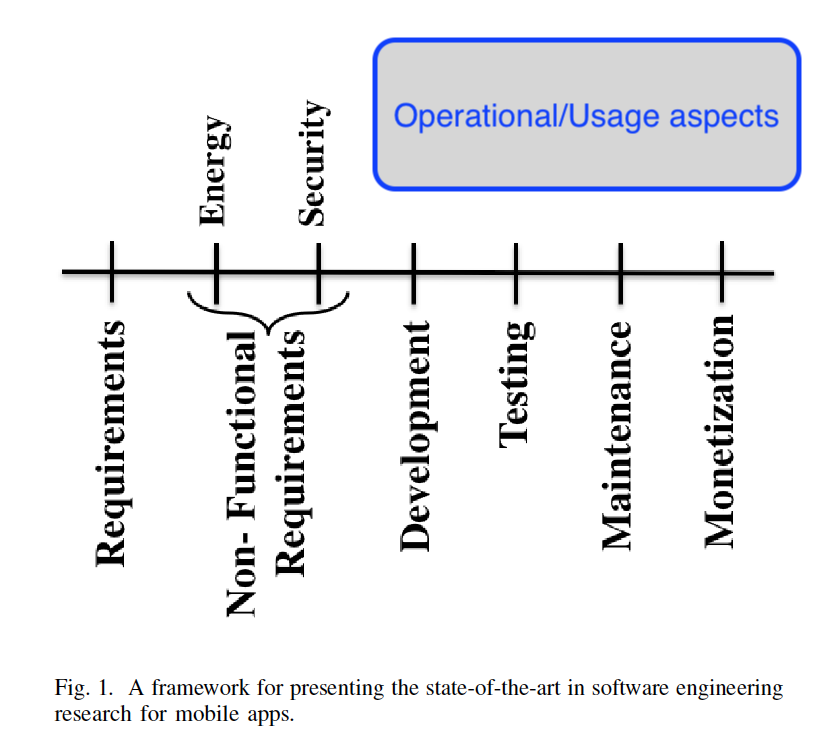
\includegraphics[width=11cm]{images/related-work/future-trends-in-sweng-for-mobile-apps-fig-1-annotated.png}
    \captionof{figure}{Annotated version of the framework for presenting the state-of-the-art in software engineering for mobile apps SANER2016~\citep{nagappan2016_future_trends_in_sw_eng_for_mobile_apps}}
    \label{fig:nagappan2016_future_trends_in_sw_eng_for_mobile_apps_figure_1_annotated}
    } % Thanks to https://tex.stackexchange.com/a/232290/88466

Mining review data for various forms of data including requests for bug fixes as is using rating as an assessment of goodness. 
Figure~\ref{fig:nagappan2016_future_trends_in_sw_eng_for_mobile_apps_figure_2_annotated} is an annotated version of their `Figure 2'. Various sources of information can be used by the development team, of these ratings and reviews are broadly researched, whereas device-level and app-level analytics have not been previously researched.

    {\centering
    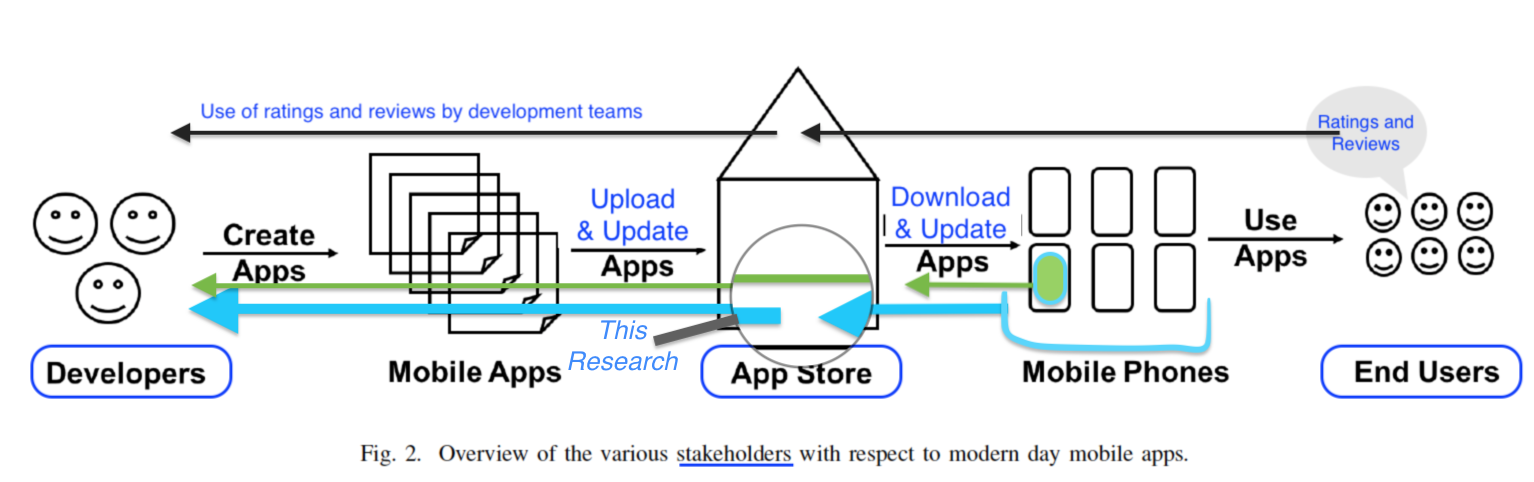
\includegraphics[width=12cm]{images/related-work/future-trends-in-sweng-for-mobile-apps-fig-2-annotated-with-highlights.png}
    \captionof{figure}{Annotated version of the various stakeholders in the modern app store ecosystemSANER2016~\citep{nagappan2016_future_trends_in_sw_eng_for_mobile_apps}}
    \label{fig:nagappan2016_future_trends_in_sw_eng_for_mobile_apps_figure_2_annotated}
    }

One of the key challenges identified is restricted access to data held by the app store, and that the only way to gather historical information is to continually mine the app store on a regular basis.

Are failure data potentially a form of requirements? (in a similar fashion to leveraging reviews in the app store to extract `requirements'). And similarly can complaints and failure data be combined to help developers prioritise issues they should consider addressing (the paper restricted the discussion to prioritising issues the developers should be \textit{testing} for).

The authors of the paper discuss limitations they experienced, perhaps without being aware that developers of Android apps have long term access to all the reviews of their apps. Details of how developers can download these and other reports, including the data structures, are available online~\citep{google_play_download_and_export_monthly_reports}. 

\emph{``Linares-Vasquez et al. [56] propose MonkeyLab, which mines recorded executions to guide the testing of Android mobile apps."} Their approach records GUI events (click events). Members of the project team (developers, testers, etc.) perform the actions, the authors claim their log collection process could scale to collecting logs from ordinary users. Key limitations include events that aren't purely dependent on the user's GUI inputs, there would also be challenges getting users to accept such an approach where the app records every input they made. Also, they generate GUI events that have x,y coordinates - absolute positioning that may have limited portability to other devices, screen rotations, and so on. Their playback also appears to require rooted devices. There are numerous other limitations described in their paper, nonetheless their work shows promise in terms of detecting and generating patterns the students did not find. It would be interesting to compare the results using accomplished software testers with experience and expertise testing similar Android apps.

Building on a point made in this paper: \emph{``the future of app quality engineering is data driven."}~\citep{maalej2016_towards_data_driven_requirements_engineering} % cite 97.

\emph{``Thus even if the app is tested on one device, there is no guarantee that it may work on another device."} - I agree. They don't provide any substance for this statement.

\emph{``The area of software maintenance is one of the most researched areas in Software Engineering. However, due to the fact that mobile apps is a young subarea within SE, the maintenance of mobile applications remains to be largely undiscovered."} - My work does investigate aspects of maintenance. 

\emph{``Syer et al. [93] compares mobile apps to larger “traditional” software systems in terms of size and time to fix defects. They find that mobile apps resemble Unix utilities, i.e., they tend to be small and developed by small groups. They also find that mobile apps tend to respond to reported defects quickly."} - Check the details of what quickly means and how the teams discovered the defects.

\emph{``Bavota et al. [16], show that the quality (in terms of change and fault-proneness) of the APIs used by Android apps negatively impacts their success, in terms of user ratings. Similarly, McDonnell et al. [65], study the stability and adoption rates for the APIs in the Android ecosystem."} - Skim read both these papers to determine their relevance.

\emph{``Another line of work examined Android-related bug reports. Bhattacharya et al. [18] study 24 mobile Android apps in order to understand the bug-fixing process. They find that mobile bug reports are of high quality, especially for security related bugs. Martie et al. [63] analyzed topics in the Android platform bugs in order to uncover the most debated topics over time. Similarly, Liu et al. [58] detected and characterized performance bugs among Android apps."} - Looks at how the bugs were fixed and compare the practices they detected with those I'm aware of. Are platform bugs that relevant? They look at performance bugs (Android Vitals also reports performance issues, Firebase Analytics has tools for performance tracking), I'm looking mainly into reliability measurements and issues.

Following on from the challenges and future directions section on maintenance research for mobile apps: do researchers focus in areas where the streetlights are rather than where the problems are? \emph{i.e.} on where they can find material to study rather than on issues that practically affect the majority of developers of apps?

\emph{``One interesting line of future research is in estimating the maintenance cost for a mobile app. Currently there are just anecdotal estimates [3]."} - Skim read this paper.

An opening gambit for my research: \emph{``Finally as mentioned in Section IX, there are several companies that collect operational data from mobile apps that have been installed on millions of devices. Most of these companies provide the app developers with the data and some rudimentary analysis on them. There is a wide variety of reliability and performance problems that can be solved by building tools and approaches that mine such operational data (past work has barely scratched the surface of such a problem by looking more at the server side of mobile applications than the client side [92])."}

Monetization is a post-release measurement, where revenues and other business-oriented metrics are applied to consider the successfulness of a mobile app. Although the paper focuses on small development teams (see the following quote as an example) in my experience many developers have measures they use in order to assess their prior work and focus their immediate future work. 
\emph{``In such apps where the development organization is small, often the developers will also have to make several engineering decisions that could affect their bottom line. Therefore software engineering researchers have examined how we can provide data to mobile app developers so that they can make these decisions in a more careful fashion."} This may be useful to support the bug triage process that developers use when determining which of the reliability bugs they choose to fix.

\emph{``Currently there are also several analytics companies (AppAnnie [1], Quettra [9], Crittercism [6] etc.) that provide valuable usage data to developers for improving their monetization strategies. They track the downloads of apps, and how the apps are being used, when users purchase things from the app etc. These companies are able to track such user data, by incorporating tracking libraries in the mobile devices. Using this information developers are able to make smarter data driven decisions with respect to making their app more successful. However, most of these recommendations are more from a marketing perspective than software engineering perspective."}
There's a lot to unpack here. Firstly although this topic discusses monetization strategies, the use of analytics can also help developers make smarter data driven decisions with respect to making their app more successful from a~\emph{software engineering} perspective. Secondly, the tracking libraries mentioned here are added to the app rather than to the device. 
\begin{itemize}
    \item AppAnnie~\citep{appannie2021}: 
    \item Crittercism: rebranded as Apteligent, which was acquired by VMWare in 2017. A few traces remain on StackOverflow and GitHub, etc. of Crittercism's analytics products of 2015. Essentially crash reporting. Some integration into enterprise systems e.g. to Splunk.
    \item Quettra: Acquired by SimilarWeb~\citep{techcrunch2015_quettra_mobile_analytics_acquired} their focus was described as a deep understanding of the users, which was then intended to help developers improve retention and also improve targeting of adverts.
\end{itemize}

\emph{``There has been some recent initial work in this direction where Bavota et al. [16] looked at the impact of using certain APIs on the ratings and Tian et al. [94] model a set of factors (like size of app, complexity of app and its UI, quality of the library code etc.) against the ratings. They were able to find that there is initial evidence that high rated apps have a certain DNA (certain value for various factors)."}


\end{mdframed}


\subsection{Sources}
\begin{itemize}
    \item \emph{What sources of analytics are available?} at a superficial level there seem to be those that operate within the app and those that are external to the app, particularly those that gather data at the platform level. I investigated a couple of widespread analytics offerings and consider several more as part of my research and understanding the overall context.
    \item \emph{How do the sources I've investigated compare in terms of the data they collect and how they are used?}
\end{itemize}

\subsection{Value}
Does using analytics provide quantitative and/or qualitative value that can be measured? Could it provide value in terms of assessing the quality of our work that was invested into developing, testing and preparing software before it was launched?
\begin{itemize}
    \item \emph{How truthy are various analytics offerings?} We discovered numerous errors in various analytics offerings. Let's share these results with the research community.
    \item \emph{How much does the fidelity matter of the analytics offerings?} Can we use the results productively even if they are flawed?
    \item \emph{How does using the various analytics compare with other sources or reflections of software quality?} Research already studies how various sources, such as ratings and reviews, can be used to identify flaws in software. Where and how do analytics fit into the larger context of these tools. \textbf{Note: I've not actively compared the sources from a practical perspective, however the catrobat case-study my be relevant}.
    \item \emph{How can the analytics be used to inform and assess our work that went into creating and testing a particular release?} data from usage analytics can reinforce aspects of what our work discovered pre-release (c.f. how Google Android's pre-launch reports cross-identify crashes) it can also identify quality flaws we missed in our work.
    \item \emph{How can analytics help with bug investigation?} a single bug instance may be hard to assess in terms of the likely scope and impact on a user-base; how, where and when can analytics help with bug investigation? We might also consider practical limits e.g. that are enforced by the real-world analytics we used. 
\end{itemize}

\subsection{Impact}
Here the focus is on whether the value has sufficient impact for anyone else to be interested in using and applying analytics. Given the nature of the research the main measures are practical, \emph{i.e.} in the real-world.
\begin{itemize}
    \item \emph{Do development teams use analytics in their practice?} If development teams find practices useful they will generally try to use them intrinsically. Do they? And if so, how?
    \item It's one thing to be able to improve a measurement such as the crash rate, it's also worth considering whether that has any material impact on other relevant measurements. \emph{Can we discern changes, even improvements, in user satisfaction, retention, etc. through using analytics?} One of the presumptions (identified in research) is that improving quality improves the user's satisfaction with mobile apps. If so, presumably we should be able to measure the effects, even crudely.
    \item \emph{Has anyone else found the work of interest? are there additional evidence of the impact of the work?} Here I'm mainly considering feedback from other researchers, and from Industry e.g. Google.
\end{itemize}

\section{My research methodology, and my choices}
As my main research question considers the application of analytics, the research needs to include a combination of usage \& analytics data where the analytics data is then applied with the intent of improving the product quality. The developers may not be successful in achieving improvements, although we hope they will be. They may also be able to improve their practices, so again their current and revised processes are also of interest.

Although I had prior experience in industry of the efficacy and potency of applying usage analytics to improve software development and testing of mobile apps, that experience is generally covered by confidentially agreements, and also the analytics tools have changed and developed markedly since those experiences. Therefore, action research seemed appropriate, particularly as one of the long-term opensource projects had extremely high failure rates according to the de-facto Android analytics tool. I decided it was appropriate and necessary to see if I could directly help that project to improve their mobile apps - \emph{``physician heal thyself"}\footnote{\href{https://en.wikipedia.org/wiki/Physician,\_heal\_thyself}{wikipedia.org/wiki/Physician,\_heal\_thyself}.}.

The next level of validity was that even if this work achieved the desired results, could other development teams achieve similar results by applying a similar approach? To help gain evidence the research engaged a separate opensource development project and development team. 

Working with non-profit opensource projects, where the teams are generally willing to make their practices and results public helps with being able to obtain information and publish the results. However, as many research projects discover, what might work for opensource projects - while important and interesting to the research community - might not matter much to the industry of professional and commercial development teams. 

Opensource apps are a tiny proportion of mobile apps available to users, so another level of learning and validation could be achieved through the insights of these professional and commercial development teams. Surveys tend to have poor response rates and lack the depth or richness I was seeking therefore I chose to engage at a deeper level as a fellow developer interviewing developers of several apps. Of course we would need the permission of their organisations, and some shared examples of their tools, their practices and their results of applying analytics well, and even times when they hadn't.

This research is not immune from also being improved, and similarly the process is likely to have plenty of scope for improvement as we learn more from the various projects, teams, apps, and analytics tools. Similarly, there is scope to find flaws, limitations, and weaknesses in the analytics tools, therefore there was scope in the research to share findings with the teams responsible for these, and related, software tools and to use the experiences and insights from any such sharing as part of this research.

Where practical, triangulation of data and analytics reports was used to help increase the confidence in the analytics and in the efficacy of using mobile analytics. As~\citep{marr2015bigdatabook} recommends:~\emph{``Measure metrics and data backed up or triangulated with other data sources."} and~\emph{``Where possible use a combination of data sets and triangulate the data. In other words, see if each data set delivers the same result so you can confirm and validate the answers."}. Triangulation of research methods is extensively covered in research. For example, \citep{fielding2012_triangulation_and_mixed_methods_designs} provides a rich discussion of triangulation and mixed methods design for various research areas. To the best of my knowledge  %SHOULD-DO decide how much to focus on triangulation, whether to discuss data triangulation as a technique for comparing analytics results (which doesn't seem to quite apply - at least in what I've read).